% Options for packages loaded elsewhere
\PassOptionsToPackage{unicode}{hyperref}
\PassOptionsToPackage{hyphens}{url}
\documentclass[
]{article}
\usepackage{xcolor}
\usepackage[margin=1in]{geometry}
\usepackage{amsmath,amssymb}
\setcounter{secnumdepth}{-\maxdimen} % remove section numbering
\usepackage{iftex}
\ifPDFTeX
  \usepackage[T1]{fontenc}
  \usepackage[utf8]{inputenc}
  \usepackage{textcomp} % provide euro and other symbols
\else % if luatex or xetex
  \usepackage{unicode-math} % this also loads fontspec
  \defaultfontfeatures{Scale=MatchLowercase}
  \defaultfontfeatures[\rmfamily]{Ligatures=TeX,Scale=1}
\fi
\usepackage{lmodern}
\ifPDFTeX\else
  % xetex/luatex font selection
\fi
% Use upquote if available, for straight quotes in verbatim environments
\IfFileExists{upquote.sty}{\usepackage{upquote}}{}
\IfFileExists{microtype.sty}{% use microtype if available
  \usepackage[]{microtype}
  \UseMicrotypeSet[protrusion]{basicmath} % disable protrusion for tt fonts
}{}
\makeatletter
\@ifundefined{KOMAClassName}{% if non-KOMA class
  \IfFileExists{parskip.sty}{%
    \usepackage{parskip}
  }{% else
    \setlength{\parindent}{0pt}
    \setlength{\parskip}{6pt plus 2pt minus 1pt}}
}{% if KOMA class
  \KOMAoptions{parskip=half}}
\makeatother
\usepackage{color}
\usepackage{fancyvrb}
\newcommand{\VerbBar}{|}
\newcommand{\VERB}{\Verb[commandchars=\\\{\}]}
\DefineVerbatimEnvironment{Highlighting}{Verbatim}{commandchars=\\\{\}}
% Add ',fontsize=\small' for more characters per line
\usepackage{framed}
\definecolor{shadecolor}{RGB}{248,248,248}
\newenvironment{Shaded}{\begin{snugshade}}{\end{snugshade}}
\newcommand{\AlertTok}[1]{\textcolor[rgb]{0.94,0.16,0.16}{#1}}
\newcommand{\AnnotationTok}[1]{\textcolor[rgb]{0.56,0.35,0.01}{\textbf{\textit{#1}}}}
\newcommand{\AttributeTok}[1]{\textcolor[rgb]{0.13,0.29,0.53}{#1}}
\newcommand{\BaseNTok}[1]{\textcolor[rgb]{0.00,0.00,0.81}{#1}}
\newcommand{\BuiltInTok}[1]{#1}
\newcommand{\CharTok}[1]{\textcolor[rgb]{0.31,0.60,0.02}{#1}}
\newcommand{\CommentTok}[1]{\textcolor[rgb]{0.56,0.35,0.01}{\textit{#1}}}
\newcommand{\CommentVarTok}[1]{\textcolor[rgb]{0.56,0.35,0.01}{\textbf{\textit{#1}}}}
\newcommand{\ConstantTok}[1]{\textcolor[rgb]{0.56,0.35,0.01}{#1}}
\newcommand{\ControlFlowTok}[1]{\textcolor[rgb]{0.13,0.29,0.53}{\textbf{#1}}}
\newcommand{\DataTypeTok}[1]{\textcolor[rgb]{0.13,0.29,0.53}{#1}}
\newcommand{\DecValTok}[1]{\textcolor[rgb]{0.00,0.00,0.81}{#1}}
\newcommand{\DocumentationTok}[1]{\textcolor[rgb]{0.56,0.35,0.01}{\textbf{\textit{#1}}}}
\newcommand{\ErrorTok}[1]{\textcolor[rgb]{0.64,0.00,0.00}{\textbf{#1}}}
\newcommand{\ExtensionTok}[1]{#1}
\newcommand{\FloatTok}[1]{\textcolor[rgb]{0.00,0.00,0.81}{#1}}
\newcommand{\FunctionTok}[1]{\textcolor[rgb]{0.13,0.29,0.53}{\textbf{#1}}}
\newcommand{\ImportTok}[1]{#1}
\newcommand{\InformationTok}[1]{\textcolor[rgb]{0.56,0.35,0.01}{\textbf{\textit{#1}}}}
\newcommand{\KeywordTok}[1]{\textcolor[rgb]{0.13,0.29,0.53}{\textbf{#1}}}
\newcommand{\NormalTok}[1]{#1}
\newcommand{\OperatorTok}[1]{\textcolor[rgb]{0.81,0.36,0.00}{\textbf{#1}}}
\newcommand{\OtherTok}[1]{\textcolor[rgb]{0.56,0.35,0.01}{#1}}
\newcommand{\PreprocessorTok}[1]{\textcolor[rgb]{0.56,0.35,0.01}{\textit{#1}}}
\newcommand{\RegionMarkerTok}[1]{#1}
\newcommand{\SpecialCharTok}[1]{\textcolor[rgb]{0.81,0.36,0.00}{\textbf{#1}}}
\newcommand{\SpecialStringTok}[1]{\textcolor[rgb]{0.31,0.60,0.02}{#1}}
\newcommand{\StringTok}[1]{\textcolor[rgb]{0.31,0.60,0.02}{#1}}
\newcommand{\VariableTok}[1]{\textcolor[rgb]{0.00,0.00,0.00}{#1}}
\newcommand{\VerbatimStringTok}[1]{\textcolor[rgb]{0.31,0.60,0.02}{#1}}
\newcommand{\WarningTok}[1]{\textcolor[rgb]{0.56,0.35,0.01}{\textbf{\textit{#1}}}}
\usepackage{graphicx}
\makeatletter
\newsavebox\pandoc@box
\newcommand*\pandocbounded[1]{% scales image to fit in text height/width
  \sbox\pandoc@box{#1}%
  \Gscale@div\@tempa{\textheight}{\dimexpr\ht\pandoc@box+\dp\pandoc@box\relax}%
  \Gscale@div\@tempb{\linewidth}{\wd\pandoc@box}%
  \ifdim\@tempb\p@<\@tempa\p@\let\@tempa\@tempb\fi% select the smaller of both
  \ifdim\@tempa\p@<\p@\scalebox{\@tempa}{\usebox\pandoc@box}%
  \else\usebox{\pandoc@box}%
  \fi%
}
% Set default figure placement to htbp
\def\fps@figure{htbp}
\makeatother
\setlength{\emergencystretch}{3em} % prevent overfull lines
\providecommand{\tightlist}{%
  \setlength{\itemsep}{0pt}\setlength{\parskip}{0pt}}
\usepackage{bookmark}
\IfFileExists{xurl.sty}{\usepackage{xurl}}{} % add URL line breaks if available
\urlstyle{same}
\hypersetup{
  pdftitle={Andmestike rühmitamine},
  pdfauthor={Allan Sims},
  hidelinks,
  pdfcreator={LaTeX via pandoc}}

\title{Andmestike rühmitamine}
\author{Allan Sims}
\date{31.01.2025}

\begin{document}
\maketitle

\section{Andmestike rühmitamine}\label{andmestike-ruxfchmitamine}

Pideva tunnuse rühmitamine tähendab andmete jaotamist gruppidesse või
kategooriatesse vastavalt nende väärtustele. See on oluline statistilise
analüüsi meetod, kui soovime analüüsida suurt hulka andmeid ning leida
seoseid või mustreid nende vahel.

Pideva tunnuse rühmitamine võib olla vajalik mitmel põhjusel:

\begin{itemize}
\item
  Andmete lihtsustamine. Pidevate tunnuste rühmitamine võib muuta andmed
  hõlpsamini tõlgendatavaks ja analüüsitavaks, eriti juhul, kui on suur
  hulk erinevaid väärtusi.
\item
  Seoste või trendide avastamine. Rühmitades pidevaid tunnuseid, võime
  avastada seoseid või mustreid erinevate gruppide vahel. See võib
  aidata mõista näiteks, kuidas üks muutuja mõjutab teist või millised
  tegurid on omavahel seotud.
\item
  Statistilise analüüsi täpsus. Pidevate tunnuste rühmitamine võib
  parandada statistiliste analüüside täpsust ja usaldusväärsust, kuna
  see võib aidata vähendada andmete varieeruvust ning korrigeerida
  võimalikke moonutusi.
\end{itemize}

Seega on pideva tunnuse rühmitamine oluline statistilise analüüsi
tööriist, mis aitab andmeid paremini mõista ja interpreteerida ning
seeläbi teha järeldusi ja otsuseid põhinevalt faktidel ja statistilistel
seostel.

\subsection{Jaotused}\label{jaotused}

\subsubsection{Empiiriline jaotus}\label{empiiriline-jaotus}

Empiiriline jaotus on statistilise andmestiku jaotus, mis põhineb
tegelikel vaatlustel või mõõtmistel. See erineb teoreetilisest
jaotusest, mis on abstraktne ja ideaalne jaotus, mida kasutatakse
statistilistes mudelites ja analüüsides.

Empiiriline jaotus saadakse andmete kogumisel ja nende analüüsimisel, et
mõista nähtuse tegelikku jaotust ja omadusi. See võib olla esitatud
graafikuna (nt histogrammina) või matemaatilise mudelina, mis kirjeldab
andmestiku jaotust.

Empiirilise jaotuse kasutamine on oluline, et saada parem arusaam
uuritavast populatsioonist või nähtusest ning teha usaldusväärseid
järeldusi statistiliste analüüside põhjal.

\subsubsection{Teoreetiline jaotus}\label{teoreetiline-jaotus}

Teoreetiline jaotus on statistikas abstraktne kontseptsioon, mis
kirjeldab tõenäosust, et mingi nähtuse väärtus võtab teatud vahemiku või
konkreetse väärtuse. Teoreetiline jaotus arvutatakse tavaliselt
matemaatiliste mudelite abil ning see aitab meil mõista andmete
tõenäosuslikku käitumist mingi statistilise populatsiooni või nähtuse
puhul. Teoreetilised jaotused on olulised statistiliste analüüside
läbiviimisel ning nende põhjal saab teha järeldusi ja prognoose
erinevate metsandustega seotud uuringute kohta.

\subsection{Histogramm}\label{histogramm}

Histogramm ehk sagedusjaotuse tulpdiagramm on graafiline esitusviis
andmehulga sageduste jaotumise näitamiseks. Histogramm koosneb üksteise
kõrvale paigutatud tulpadest, kus iga tulp esindab teatud vahemikku või
klassi, ning selle kõrgus näitab antud klassi sagedust. Horisontaaltelg
esitab klasside vahemikke või kategooriaid ning vertikaaltelg näitab
vastavate klasside sagedusi või sageduste suhtarvu. Histogrammi abil
saab hinnata andmehulga jaotust ning tuvastada erinevaid tendentse ja
mustreid andmetes. Histogrammi loomise eesmärgiks on anda visuaalne
ülevaade andmete koondumisest ja levikust ning seeläbi paremini mõista
andmete struktuuri. Histogrammi loomisel on oluline valida sobiv
klassilaius, mis võimaldab õigesti tõlgendada ja analüüsida andmeid.
Histogramm on oluline tööriist statistilise info esitamiseks ja
mõistmiseks nii akadeemilistes kui ka praktilistes seadetes, sealhulgas
metsanduses.

\begin{example}
Olgu juhuslikuks suuruseks puu diameeter. Antud näites on esitatud
Järvseljal kvartalis 252 kasvanud 75 aasta vanuse naadisaariku
saarepuude diameetri empiiriline jaotus proovitüki kluppimisandmete
järgi.
\end{example}

\subsubsection{R keskkonnas:}\label{r-keskkonnas}

\begin{Shaded}
\begin{Highlighting}[]
\CommentTok{\# Näide R keskkonnas}
\CommentTok{\# Laadime peatükis kasutatavad paketid}
\FunctionTok{library}\NormalTok{(dplyr)}
\FunctionTok{library}\NormalTok{(ggplot2)}
\end{Highlighting}
\end{Shaded}

Esmalt loome pidevast tunnusest mõned juhuslikud andmed ning seejärel
kuvame nende andmete põhjal histogrammi.

\textbf{Histogramm}

\begin{Shaded}
\begin{Highlighting}[]
\CommentTok{\# Laadime proovitükkide andmed}
\NormalTok{df }\OtherTok{\textless{}{-}}\NormalTok{ readxl}\SpecialCharTok{::}\FunctionTok{read\_excel}\NormalTok{(}\StringTok{"data/naited.xlsx"}\NormalTok{,}\StringTok{"prt\_andmed"}\NormalTok{)}

\CommentTok{\# koostame diameetrite histogrammi}
\FunctionTok{ggplot}\NormalTok{(df, }\FunctionTok{aes}\NormalTok{(d)) }\SpecialCharTok{+}
  \FunctionTok{geom\_histogram}\NormalTok{(}
    \FunctionTok{aes}\NormalTok{(}\AttributeTok{y =} \FunctionTok{after\_stat}\NormalTok{(density)),}
    \AttributeTok{bins =} \DecValTok{15}\NormalTok{,}
    \AttributeTok{fill =} \StringTok{"white"}\NormalTok{,}
    \AttributeTok{color =} \StringTok{"black"}
\NormalTok{  ) }\SpecialCharTok{+}
  \FunctionTok{geom\_density}\NormalTok{(}\AttributeTok{color =} \StringTok{"red"}\NormalTok{, }\AttributeTok{lwd =} \DecValTok{1}\NormalTok{) }\SpecialCharTok{+}
  \FunctionTok{labs}\NormalTok{(}\AttributeTok{y =} \StringTok{"f(x)"}\NormalTok{)}
\end{Highlighting}
\end{Shaded}

\begin{figure}
\centering
\pandocbounded{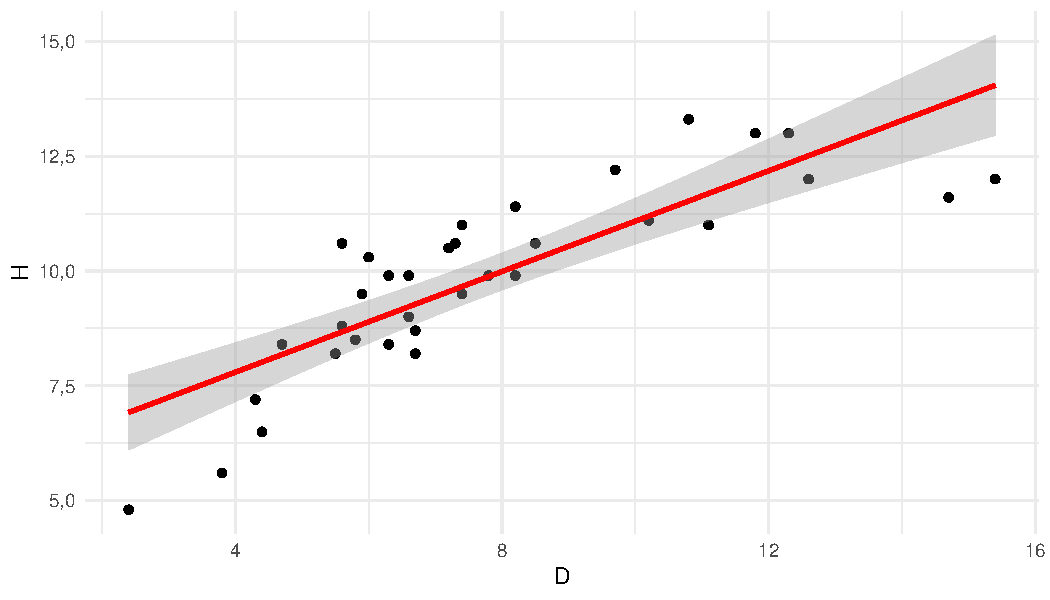
\includegraphics[keepaspectratio]{03-ruhmitamine_files/figure-latex/unnamed-chunk-4-1.pdf}}
\caption{Histogramm}
\end{figure}

See kood loob R-keeles \texttt{ggplot2} paketiga graafiku, mis
visualiseerib andmete jaotust. Vaatame seda samm-sammult:

\begin{enumerate}
\def\labelenumi{\arabic{enumi}.}
\item
  \textbf{\texttt{ggplot(df,\ aes(x))}}: See alustab graafiku loomist.
  \texttt{df} on andmetabel, mis sisaldab andmeid. \texttt{aes(x)}
  määrab, et x-teljele kuvatakse muutujat \texttt{x}. See on graafiku
  ``põhi'', millele järgnevad kihid lisatakse.
\item
  \textbf{\texttt{geom\_histogram(...)}}: See lisab histogrammi.

  \begin{itemize}
  \tightlist
  \item
    \texttt{geom\_histogram()} funktsioon loob histogrammi, mis näitab
    andmete sagedust erinevatesse gruppidesse jaotatuna.
  \item
    \texttt{aes(y=after\_stat(density))} on oluline osa. See määrab, et
    y-teljel kuvatakse \emph{tihedust} (density), mitte lihtsalt
    sagedust (count). \texttt{after\_stat()} funktsiooniga pääsetakse
    ligi statistilisele väärtusele, mis arvutatakse histogrammi
    joonistamisel. Tihedus on normaliseeritud sagedus, nii et
    histogrammi pindala on 1. See võimaldab histogrammi ja
    tihedusfunktsiooni kõrvuti kuvada.
  \item
    \texttt{fill="white"} määrab histogrammi kastide sisemise värvi
    valgeks.
  \item
    \texttt{color="black"} määrab histogrammi kastide piirjoone värvi
    mustaks.
  \end{itemize}
\item
  \textbf{\texttt{geom\_density(color="red",\ lwd=1)}}: See lisab
  tihedusfunktsiooni graafikule.

  \begin{itemize}
  \tightlist
  \item
    \texttt{geom\_density()} funktsioon arvutab ja joonistab andmete
    tihedusfunktsiooni, mis on silutud kõver, mis näitab andmete jaotuse
    kuju.
  \item
    \texttt{color="red"} määrab tihedusfunktsiooni joone värvi punaseks.
  \item
    \texttt{lwd=1} määrab joone paksuse (line width) 1-ks.
  \end{itemize}
\item
  \textbf{\texttt{labs(y\ =\ "f(x)")}}: See lisab y-teljele sildi
  ``f(x)''. See on hea tava, et telgi selgelt märgistada, eriti kui
  y-telg näitab tihedust, mitte sagedust. ``f(x)'' on levinud tähistus
  tõenäosustihedusfunktsioonile (probability density function).
\end{enumerate}

\textbf{Sageduste arvutamine}

Tulpdiagrammile võib eelnevalt välja arvutada antud sagedused. Selleks
saab kasutada funktsiooni \texttt{cut()}, mis vajab rühmade piire
sisendiks ning seejärel saab juba funktsiooniga \texttt{table()}
loendada kokku iga rühma liikmete arvu.

\subsubsection{Exceli keskkonnas:}\label{exceli-keskkonnas}

\paragraph{Histogramm}\label{histogramm-1}

Histogrammi loomiseks Excelis peab andmed esmalt sisestama tabelisse ja
seejärel kasutama selle jaoks sobivat tööriista.

\begin{enumerate}
\def\labelenumi{\arabic{enumi}.}
\tightlist
\item
  Sisesta pideva tunnuse väärtused Exceli tabelisse.
\item
  Vali need lahtrid, kuhu soovid luua histogrammi.
\item
  Mine menüüsse ``Lisa'' ja vali ``Diagramm''.
\item
  Vali ``Histogramm'' ja klikka ``OK''.
\item
  Seejärel on võimalik vormindada telje suvandeid, millega määratakse
  rühmade (MS Exceli keskkonnas nimetusega ``salv'') parameetrid.
\end{enumerate}

\paragraph{Sageduste arvutamine}\label{sageduste-arvutamine}

MS Exceli funktsioon \texttt{FREQUENCY()} võimaldab kasutajatel määrata,
kui sageli väärtused esinevad teatud väärtusvahemikes. See funktsioon
sobib hästi suurte andmekogumite analüüsimiseks, et mõista andmete
jaotust ilma iga üksiku väärtuse manuaalse üle vaatamiseta.

Enne \texttt{FREQUENCY()} funktsiooni kasutamist peate määrama rühmade
vahemike piirid, millesse soovite oma andmed jaotada. Need piirid tuleks
sisestada eraldi veergu Exceli töölehel. Näiteks, kui soovite analüüsida
testitulemusi vahemikus 0-100, võite määrata piirid 0, 20, 40, 60, 80,
100.

\begin{enumerate}
\def\labelenumi{\arabic{enumi}.}
\tightlist
\item
  \textbf{Andmete ja piiride sisestamine:}
\end{enumerate}

\begin{itemize}
\tightlist
\item
  Sisestage oma andmekogum ühte veergu (nt A2:A101).
\item
  Sisestage vahemike piirid teise veergu (nt B2:B7, eeldades, et
  esitasite näiteks eelmises punktis toodud piirid).
\end{itemize}

\begin{enumerate}
\def\labelenumi{\arabic{enumi}.}
\setcounter{enumi}{1}
\tightlist
\item
  \textbf{Funktsiooni rakendamine:}
\end{enumerate}

\begin{itemize}
\tightlist
\item
  Valige tühi ala, kuhu soovite tulemused väljastada. Sellel peaks olema
  sama palju lahtrid kui määratletud vahemike piire. Kui teil on 6
  piiri, valige 6 lahtrit vertikaalselt.
\item
  Sisestage \texttt{FREQUENCY()} funktsioon. Kuna \texttt{FREQUENCY()}
  on massiivifunktsioon, tuleb see sisestada massiivivalemiga. Algusesse
  minev andmevahemik on teie andmekogum ja teine vahemik on teie
  vahemike piirid. Näiteks: \texttt{=FREQUENCY(A2:A101,\ B2:B7)}
\item
  Pärast funktsiooni sisestamist lõpetage sisestus, vajutades
  \textbf{Ctrl+Shift+Enter}. Excel käitab nüüd \texttt{FREQUENCY()}
  funktsiooni massiivina ja täidab valitud lahtrid andmete sagedustega,
  mis vastavad määratud vahemikele.
\end{itemize}

\end{document}
